\section{背景}

本节首先在 \S\ref{sec:background_rl} 中介绍智能体 RL 的训练流程；随后在 \S\ref{sec:background_resource} 中讨论外部资源管理问题；再在 \S\ref{sec:background_op} 中分析过量预留现象；最后在 \S\ref{sec:background_opp} 中总结我们看到的机会与挑战。

\subsection{智能体 RL 训练}
\label{sec:background_rl}
智能体在 AI 编程、深度搜索和具身智能等现实任务中表现出明显的性能优势~\citep{dou2024stepcoder,qi2025webrl,wang2023voyager}。与传统 LLM 不同，智能体 LLM 会通过 shell 命令、API 或设备操作等外部工具与真实世界交互。这种工具使用方式使得智能体 LLM 的 RL 流水线与传统 LLM 显著不同。

\begin{figure}[t]
    \centerline{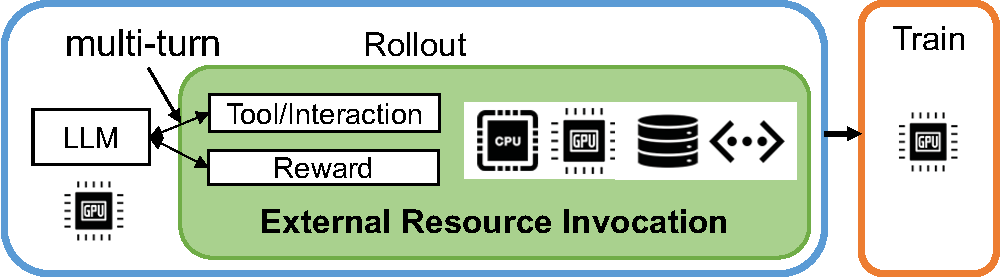
\includegraphics[width=0.7\linewidth]{figures/background_workflow.pdf}}
    \vspace{-0.1in}
    \caption{智能体 RL 的一次训练 step。}
    \label{fig:background_workflow}
    \vspace{-0.2in}
\end{figure}

如图~\ref{fig:background_workflow} 所示，给定一个 batch 的样本后，RL 框架首先使用智能体 LLM 处理这些样本并收集执行轨迹，这一阶段在 RL 中通常称为 \textit{rollout}。在 rollout 期间，框架通常遵循 ReAct 模式~\citep{yao2022react}：LLM 根据输入提示决定如何使用工具，随后 RL 框架执行相应工具调用并接收环境观测。轨迹结束后，系统会基于偏好信号（如 RLHF~\citep{ouyang2022training} 和 LLM-as-a-judge~\citep{bai2022constitutional}）或基于真值信号（如 RLVR~\citep{guo2025deepseek}）计算奖励，并据此训练 LLM。

在一条轨迹内部，智能体 RL 往往会多轮重复 ReAct 模式，以提升模型的工具使用能力。虽然 LLM 的生成与训练主要消耗 GPU，但工具调用会依赖 CPU、GPU、存储和网络等异构资源。从 RL 框架视角看，这些位于训练系统之外的资源统称为 \textbf{外部资源}。频繁使用外部资源正是智能体 RL 的典型特征。例如 AI 编程会反复通过 CPU 执行 shell 命令或编辑文件，而 DeepSearch 会频繁访问网站并消耗 API 配额。除此之外，轨迹结束时的奖励计算往往也依赖外部资源，例如 LLM-as-a-judge 常被部署为独立模型服务，而 AI 编程任务的奖励评估需要运行大量测试用例。凡是发生在 RL 框架之外、需要调用额外资源的操作，都可以统一称为 \textbf{外部资源调用}。

\subsection{外部资源管理}
\label{sec:background_resource}
智能体 RL 训练依赖外部资源来承载环境、工具或奖励服务，因此对这些外部资源的管理会直接影响 RL 效率与成本。

第一，RL 任务的效率高度依赖外部资源使用是否合理。如果外部资源不足，或者资源分配不合适，外部调用的执行时长就会增加。根据 \S\ref{sec:background_rl} 中的常见工作流，这些外部调用都位于 rollout 的关键路径上，因此更长的调用意味着更慢的 rollout，也意味着更慢的 RL 训练。图~\ref{fig:motiv_sm}(a) 展示了同一 RL 任务在不同外部资源规模下的对比：当资源不足（仅 0.5$\times$）时，平均 ACT 和 step 时长都明显高于资源充足（1$\times$）的情况。更严重的是，若外部调用失败过多，整个 RL 训练任务也可能失败~\citep{jiang2025verltool}。

第二，外部调用会带来额外资源成本，因此降低这部分成本同样很关键。实际中，智能体 RL 往往需要部署 CPU 集群来构建环境，或部署专用 GPU 运行奖励服务，这些都会产生额外费用。例如 MOPD~\citep{xiao2026mimo} 这样的蒸馏流程，为了给单个 RL 任务打分，可能需要数十个教师模型和数百张 GPU。然而这些外部 GPU 并没有被充分利用。图~\ref{fig:motiv_sm}(b) 给出了 12 个教师模型对应 GPU 的 SM 活跃度，可以看到它在时间维度与模型维度上都大幅波动，平均值甚至不到 3\%，说明外部资源浪费极为严重。

\begin{figure}[t]
    \begin{minipage}{0.24\linewidth}
        \centerline{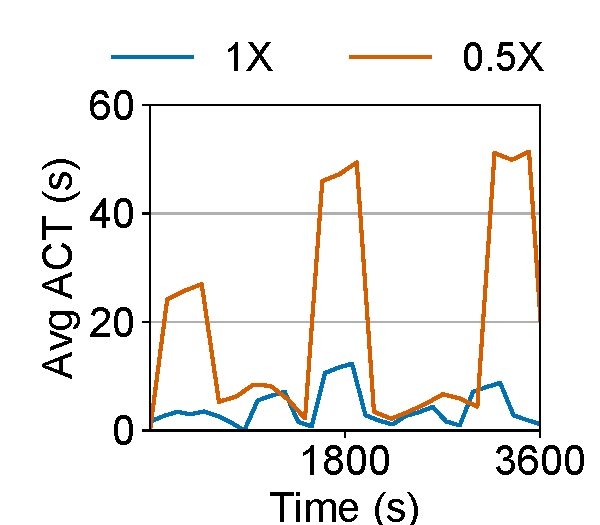
\includegraphics[width=\linewidth]{figures/Motiv_code_act.pdf}}
        \centerline{\small \quad(a)}
    \end{minipage}
    \begin{minipage}{0.24\linewidth}
        \centerline{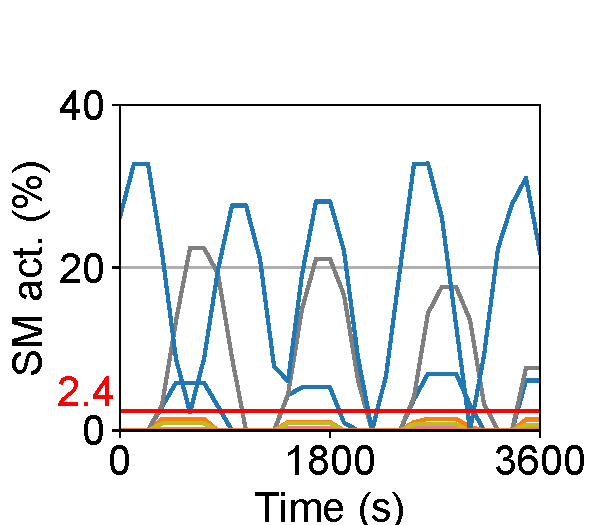
\includegraphics[width=\linewidth]{figures/Motiv_mopd_sm.pdf}}
        \centerline{\small \quad(b)}
    \end{minipage}
    \begin{minipage}{0.24\linewidth}
        \centerline{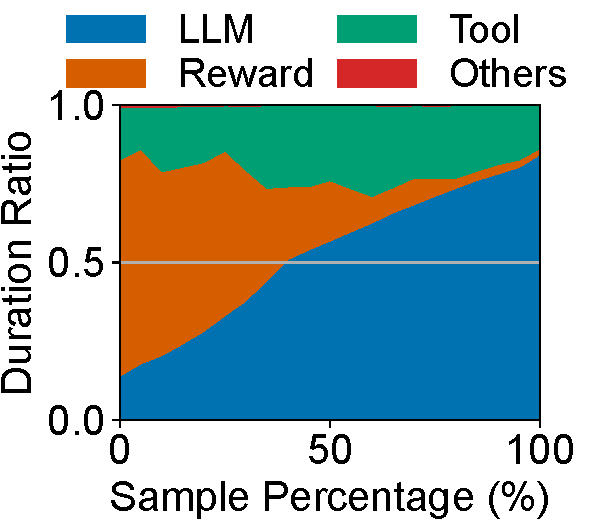
\includegraphics[width=\linewidth]{figures/Motiv_traj_code.pdf}}
        \centerline{\small \quad(c)}
    \end{minipage}
    \begin{minipage}{0.24\linewidth}
        \centerline{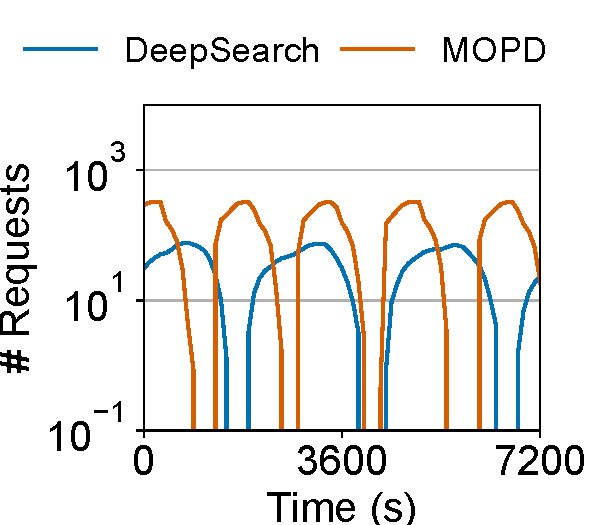
\includegraphics[width=\linewidth]{figures/Motiv_req_counts.pdf}}
        \centerline{\small \quad(d)}
    \end{minipage}
    \vspace{-0.1in}
    \caption{(a) 在 1$\times$ 与 0.5$\times$ 外部资源规模下的平均 ACT；(b) MOPD 中 12 个奖励服务的 SM 活跃度；(c) 代码智能体 rollout 时长占比；(d) 两个智能体 RL 任务中的外部调用次数。}
    \label{fig:motiv_sm}
    \vspace{-0.2in}
\end{figure}

\subsection{外部资源的过量预留}
\label{sec:background_op}

\parabf{轨迹内部的过量预留。}
在智能体 RL 中，LLM 生成与外部调用会在轨迹内部交替进行，但现有系统通常会在 rollout 开始时就创建环境并长期保留相应外部资源，直到整条轨迹结束才释放。结果是，这些被预留的资源在大部分时间里都处于空闲状态，本可以被其他轨迹复用。以 AI 编程为例，图~\ref{fig:motiv_sm}(c) 表明被浪费的外部资源可占到 53\%。在有限外部资源条件下，这种轨迹内部过量预留会显著限制系统并发、增加工具调用排队延迟，并阻碍系统为计算密集型操作动态追加资源，从而拉长 rollout 时间、降低 RL 框架整体效率，也降低训练集群中 GPU 的利用率。

\parabf{RL 任务内部的过量预留。}
在任务层面，不同 RL 任务往往需要不同的外部服务来完成交互或奖励计算，因为服务类型和配置都可能不同~\citep{li2025cuda,jin2025search,xiao2026mimo}。例如，不同任务使用的奖励模型可能架构或参数不同，因此通常会被部署在彼此隔离的资源上~\citep{micromulti,jiang2025verltool}。但这些服务并不是一直都处于高负载状态。对于单个 RL 任务来说，在训练阶段甚至根本不会发生外部调用，因此预留出来的外部服务会长时间闲置。图~\ref{fig:motiv_sm}(d) 展示了 DeepSearch 与 MOPD 两个真实智能体 RL 任务中的外部调用次数，其数量变化可以达到三个数量级，因此会造成严重的外部资源浪费。

\subsection{机会与挑战}
\label{sec:background_opp}

\parabf{动作级调度带来的机会。}
为了应对上述过量预留导致的低效，我们提出在 \textbf{动作级} 管理外部资源。这里的 \textit{action} 指一次原子化的外部资源调用，在其执行期间，轨迹中不会穿插 LLM 生成或其他动作。不同于让每条轨迹各自占有资源并独立完成调用，动作级方案把所有动作提交到统一系统中进行集中调度。系统会把寿命较长的环境或服务占用拆解成动作级占用，也就是 \textbf{Breakdown}；同时，它会对同类资源进行池化，并在动作之间弹性分配，也就是 \textbf{Pool}。通过 \textbf{Breakdown} 与 \textbf{Pool}，系统能够在空闲时释放或缩减资源，从而消除过去由于轨迹内 LLM 生成阶段或任务内训练阶段造成的过量预留。除此之外，动作级调度还带来了更灵活、更细粒度的资源分配能力。当资源充足时，它可以为弹性动作动态分配更多资源单元，提高并行度（DoP），从而缩短执行时长，进一步提升整体 RL 训练效率。

概括来看，把资源管理粒度从轨迹或 RL 任务下沉到单个动作，可以带来两点好处：(i) 通过跨轨迹、跨任务复用，减少长空闲期造成的资源闲置；(ii) 通过动态扩缩容，降低与外部环境交互的延迟。

\parabf{挑战。}
尽管动作级调度带来了明确机会，但它也面临多项挑战。首先，不同动作可能同时依赖多种资源，并且不同资源在容量、约束和可扩展性上都不同，因此需要统一的动作建模。其次，调度算法需要在极短时间窗口内完成决策，否则调度本身的开销就会抵消收益。最后，不同资源具有截然不同的拓扑和执行特性，例如 CPU 集群、GPU 集群和外部 API 配额都不能用同一种方式管理，因此还需要与统一调度器协同工作的异构资源管理器。
